% Standalone: bandwidth--safety four-stage chain
\documentclass[tikz,border=6pt]{standalone}
\usepackage{amsmath}
\usetikzlibrary{arrows.meta,positioning}
\begin{document}
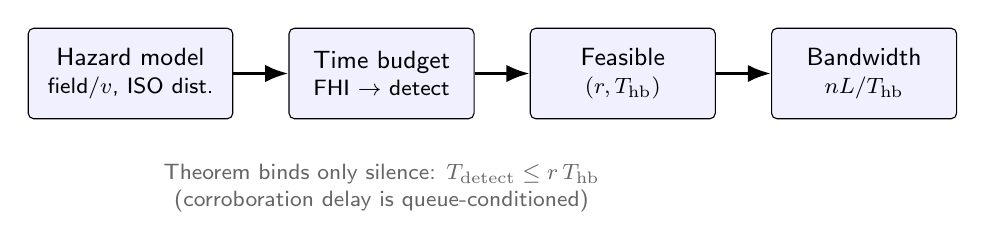
\begin{tikzpicture}[
  font=\sffamily\small,
  st/.style={draw, rounded corners=2pt, align=center, inner sep=7pt, minimum width=2.35cm, minimum height=1.15cm, fill=blue!6},
  arr/.style={-{Latex}, very thick},
]
\node[st] (a) {Hazard model\\[-1pt]{\footnotesize field$/v$, ISO dist.}};
\node[st, right=0.7cm of a] (b) {Time budget\\[-1pt]{\footnotesize FHI $\to$ detect}};
\node[st, right=0.7cm of b] (c) {Feasible\\[-1pt]{\footnotesize $(r,T_{\mathrm{hb}})$}};
\node[st, right=0.7cm of c] (d) {Bandwidth\\[-1pt]{\footnotesize $nL/T_{\mathrm{hb}}$}};
\draw[arr] (a) -- (b);
\draw[arr] (b) -- (c);
\draw[arr] (c) -- (d);
\node[below=0.45cm of b, font=\sffamily\footnotesize, text=black!60, align=center] {%
  Theorem binds only silence: $T_{\mathrm{detect}}\le r\,T_{\mathrm{hb}}$\\
  (corroboration delay is queue-conditioned)};
\end{tikzpicture}
\end{document}
